\documentclass[12pt,a4paper]{article}

\usepackage[margin=2.2cm]{geometry}
\usepackage{fontspec}
\usepackage{xeCJK}
\setmainfont{Times New Roman}
\setCJKmainfont{DFKai-SB}[AutoFakeBold,AutoFakeSlant]
\setCJKmonofont{DFKai-SB}
\usepackage{amsmath,amssymb,bm}
\usepackage{booktabs}
\usepackage{graphicx}
\usepackage{caption}
\usepackage{setspace}
\captionsetup{font=small,labelfont=bf,skip=4pt}
\graphicspath{{figures/}}
\usepackage{hyperref}
\setstretch{1.08}
\raggedbottom

\hypersetup{colorlinks=true,linkcolor=black,urlcolor=blue}

\title{\textbf{Control System Homework 03}\\[0.35em]
\large 延伸探討：台車倒立擺的實數右半平面零點與下衝\\[0.35em]
\normalsize （原題為第 46 題；延伸另編為延伸一、延伸二、延伸三）}
\author{許楷翊 \quad B13901040}
\date{2026 年 10 月}

\begin{document}
\maketitle

\section*{延伸問題}

為了把抽象的右半平面零點接到看得到的物理現象，本份回答下面三題。
原作業第 46 題的小題仍稱「第 46 題 (a)」「第 46 題 (b)」「第 46 題 (c)」。
延伸題目原本也寫成 (a)(b)(c)；為避免和原題撞號，本文改稱延伸一、延伸二、延伸三。

\begin{enumerate}
  \item[\textbf{延伸一.}]
  \textbf{建立物理模型與數學連結。}
  尋找或推導一個現實中具有單一實數右半平面零點的經典動力學系統
  （例如台車上的倒立擺、後輪轉向的載具，或在指尖上平衡直尺）。
  寫下簡化後的線性化運動方程式，推導轉移函數，明確求出極點與零點，
  並證明實數右半平面零點的個數是奇數，符合第 46 題必定產生下衝的條件。

  \item[\textbf{延伸二.}]
  \textbf{VPython 三維視覺化模擬。}
  用 VPython 建立上述系統的三維動畫。初始狀態為靜止，\(t>0\) 給予正向的目標步階命令。
  動畫要看得到物體的軌跡與姿態。視窗中同步畫出輸出（例如台車位置）隨時間的曲線，以便和動畫對照。

  \item[\textbf{延伸三.}]
  \textbf{物理直觀與動態行為。}
  綜合推導與模擬：描述步階命令剛下達時，系統如何具體走出圖上「往錯誤方向」的下衝；
  再用慣性、力矩平衡、重心轉移說明，為什麼必須先往反方向，才能最後朝目標前進；
  若沒有這個初始反向動作，物理狀態會出什麼問題。
\end{enumerate}

選定的系統是台車倒立擺。三維動畫程式是 \texttt{inverted\_pendulum\_undershoot.py}，
影片在 \url{https://youtu.be/Q5fvMPvR5O4}。

參數後文都固定用這一組，和程式相同：
\[
  M=1.0\,\mathrm{kg},\quad
  m=0.25\,\mathrm{kg},\quad
  L=1.5\,\mathrm{m},\quad
  g=9.81\,\mathrm{m/s^2}.
\]

%==============================================================================
\section{延伸一　物理模型與數學連結}

\subsection{線性化運動方程式}

台車在水平軌道上，位置 \(x\) 向右為正，外力 \(F\) 也向右為正。
擺桿長度 \(L\)，質量集中在末端。
\(\theta=0\) 是鉛直向上；\(\theta>0\) 表示擺錘在支點的右側，也就是偏向 \(+x\)。

擺錘座標
\[
  x_b=x+L\sin\theta,\qquad y_b=L\cos\theta
\]
（\(y\) 向上，支點高度取 0）。位能 \(mgy_b=mgL\cos\theta\) 在 \(\theta=0\) 最大，所以正立是不穩定平衡。

動能與位能寫成拉格朗日
\[
  \mathcal{L}
  =\frac12(M+m)\dot x^2
   +mL\dot x\dot\theta\cos\theta
   +\frac12 mL^2\dot\theta^2
   -mgL\cos\theta.
\]
對 \(x\)、\(\theta\) 各做一次 Euler--Lagrange，得到還沒線性化的式子
\begin{align}
  (M+m)\ddot x+mL\ddot\theta\cos\theta-mL\dot\theta^2\sin\theta&=F,
  \label{eq:nl-x}\\
  \ddot x\cos\theta+L\ddot\theta-g\sin\theta&=0.
  \label{eq:nl-th}
\end{align}
程式積分的就是這兩條。

在 \(\theta=0\) 附近，\(\sin\theta\approx\theta\)、\(\cos\theta\approx 1\)，含 \(\dot\theta^2\) 的項是二階，丟掉。線性化運動方程式是
\begin{align}
  (M+m)\ddot x+mL\ddot\theta&=F,
  \label{eq:lin-x}\\
  \ddot x+L\ddot\theta-g\theta&=0.
  \label{eq:lin-th}
\end{align}
第二式在台車固定（\(\ddot x=0\)）時變成 \(\ddot\theta=(g/L)\theta\)。
偏離直立的角度會以 \(e^{+\sqrt{g/L}\,t}\) 散開。這個成長率和下面的右半平面零點是同一個數。

%==============================================================================
\subsection{開迴路轉移函數}

對 \eqref{eq:lin-x}、\eqref{eq:lin-th} 做拉普拉斯轉換：
\begin{align}
  (M+m)s^2X+mLs^2\Theta&=F,
  \label{eq:s-x}\\
  s^2X+(Ls^2-g)\Theta&=0.
  \label{eq:s-th}
\end{align}
由 \eqref{eq:s-th}，
\[
  \Theta=\frac{s^2X}{g-Ls^2}.
\]
代回 \eqref{eq:s-x}，整理後
\begin{equation}
  G(s)=\frac{X(s)}{F(s)}
  =\frac{g-Ls^2}{s^2\bigl[(M+m)g-MLs^2\bigr]}
  =\frac{s^2-g/L}{Ms^2\bigl(s^2-(M+m)g/(ML)\bigr)}.
  \label{eq:G}
\end{equation}
分子 \(s^2-g/L=(s-\sqrt{g/L})(s+\sqrt{g/L})\)。
零點是
\begin{equation}
  s=\pm\sqrt{\frac{g}{L}}=\pm\sqrt{6.54}\approx\pm 2.557.
  \label{eq:zeros}
\end{equation}
其中只有 \(+\sqrt{g/L}\) 在右半平面，而且是實數。沒有成對的複數零點。
所以開迴路實數右半平面零點的個數是 \(1\)，是奇數。

極點來自分母：
\begin{equation}
  s=0\ (\text{二重}),\qquad
  s=\pm\sqrt{\frac{(M+m)g}{ML}}
   =\pm\sqrt{8.175}\approx\pm 2.859.
  \label{eq:ol-poles}
\end{equation}
\(+\sqrt{(M+m)g/(ML)}\) 在右半平面，原點還有兩個極點。開迴路不穩定。

有兩件事要分開看。零點的位置 \(\sqrt{g/L}\) 與台車質量、擺錘質量都無關，只看擺長和重力；它就是台車卡住時，角度發散的那個指數。
極點則會被 \(M\)、\(m\) 搬走。開迴路已經是嚴格真分（分母比分子高兩次），但第 46 題 (c) 還要求穩定。這裡有一個右半平面極點，原點的極點也讓直流增益不存在，所以不能從 \(G(s)\) 直接說步階一定下衝。這件事留到下面的閉迴路再套第 46 題 (c)。

\subsection{閉迴路：零點留著，極點移走}

令狀態為 \((x,\dot x,\theta,\dot\theta)\)。模擬用的控制律是線性狀態回授加位置命令 \(r\)，
\begin{equation}
  F=-k_x(x-r)-k_v\dot x-k_\theta\theta-k_\omega\dot\theta,
  \label{eq:u}
\end{equation}
極點放在
\[
  -3.5,\ -4,\ -4.8,\ -5.6.
\]
特徵多項式
\begin{align}
  \chi(s)&=(s+3.5)(s+4)(s+4.8)(s+5.6) \nonumber\\
         &=s^4+17.9s^3+118.88s^2+347.2s+376.32.
  \label{eq:chi}
\end{align}
四個根的實部都是負的，閉迴路穩定。

狀態回授不改變從 \(F\) 到 \(x\) 的傳輸零點，也不改變相對次數 \(2\) 的高頻係數。
開迴路 \(s^2G(s)\to 1/M=1\)，回授之後仍然
\[
  \frac{X(s)}{F(s)}=\frac{s^2-g/L}{\chi(s)}.
\]
命令從 \eqref{eq:u} 的 \(+k_x r\) 進來。把這一項的係數記成 \(N\)（程式裡 \(N=k_x\)），則
\begin{equation}
  T(s)=\frac{X(s)}{R(s)}=N\,\frac{s^2-g/L}{\chi(s)}.
  \label{eq:T}
\end{equation}
\(T(s)\) 的零點仍是 \(\pm\sqrt{g/L}\)。要讓直流增益為 \(1\)（停在命令的那個位置），
\[
  T(0)=N\frac{-g/L}{\chi(0)}=1.
\]
穩定的首一多項式可以拆成 \((s+a)\) 和 \(s^2+bs+c\)，係數都是正的，所以 \(\chi(0)>0\)。因此
\begin{equation}
  N=-\chi(0)\,\frac{L}{g}
   =-376.32\times\frac{1.5}{9.81}
   =-57.541<0.
  \label{eq:N}
\end{equation}
位置增益是負的，不是算錯。代回去，
\begin{equation}
  T(s)=\frac{-57.541\,s^2+376.32}{s^4+17.9s^3+118.88s^2+347.2s+376.32}
      =-57.541\,\frac{(s-2.557)(s+2.557)}{\chi(s)}.
  \label{eq:Tnum}
\end{equation}
右半平面上的實數零點還是只有 \(s=+2.557\) 一個。
\(-2.557\) 在左半平面。分母次數 \(4\)、分子次數 \(2\)，嚴格真分。

這三條（穩定、嚴格真分、奇數個實數右半平面零點）就是第 46 題 (c) 的假設。
單位步階的穩態是 \(T(0)=1>0\)，一開始卻必須往負的方向走。

把「一開始」寫具體一點，就對上第 46 題 (c) 的定義，不是第 46 題 (a) 要畫的 \(G_1\)、\(G_2\) 草圖。
相對次數是 \(2\)，所以 \(x(0)=\dot x(0)=0\)，第一個不是零的導數是
\[
  \ddot x(0^+)=\lim_{s\to\infty}s^2T(s)=N=-57.541<0.
\]
穩態在 \(+1\,\mathrm{m}\)，初始加速度卻是負的：響應一開始往錯的方向。
這個符號只靠 \(\chi(0)>0\) 和零點 \(\pm\sqrt{g/L}\)，不靠這四個極點具體放在哪。
只要閉迴路穩定、直流增益為正，步階一開始都會先往 \(-x\)。

%==============================================================================
\section{延伸二　模擬軌跡}

這一節只記錄動畫裡的軌跡，用來供給延伸三對照。它不是第 46 題 (b)：原題 (b) 問的是 \(G_1\) 與 \(G_2\) 的暫態為什麼不同。

程式從靜止 \((x,\dot x,\theta,\dot\theta)=(0,0,0,0)\) 開始，先停到 \(t=0\)，再把命令切成 \(r=+1\,\mathrm{m}\)。
積分用的是 \eqref{eq:nl-x}、\eqref{eq:nl-th}，不是線性式；控制器才是上面這組線性增益。
畫面上台車、擺桿角度、地面軌跡一起在動，旁邊的 \(x(t)\) 用同一條時間軸往右畫。\(\theta(t)\) 另開一張圖。
這段三維演示錄在 \url{https://youtu.be/Q5fvMPvR5O4}：步階一下達，力箭頭先指向 \(-x\)，台車與青色軌跡先往左，擺錘同時倒向目標。

非線性軌跡的幾個點：

\begin{center}
\begin{tabular}{@{}cccc@{}}
\toprule
\(t\) (s) & \(x\) (m) & \(\theta\) (deg) & \(F\) (N) \\
\midrule
\(0^+\)   & \(0\)      & \(0\)        & \(-57.5\) \\
\(0.05\)  & \(-0.053\) & \(+2.0\)     & \(-18.1\) \\
\(0.20\)  & \(-0.318\) & \(+12.7\)    & \(+17.6\) \\
\(0.25\)  & \(-0.343\) & \(+14.1\)    & \(+17.8\) \\
\(0.50\)  & \(+0.024\) & \(+6.7\)     & \(+1.2\) \\
\(1.0\)   & \(+0.829\) & \(-6.5\)     & \(-3.0\) \\
\(4.0\)   & \(+1.000\) & \(\approx 0\) & \(\approx 0\) \\
\bottomrule
\end{tabular}
\end{center}

\begin{figure}[ht]
  \centering
  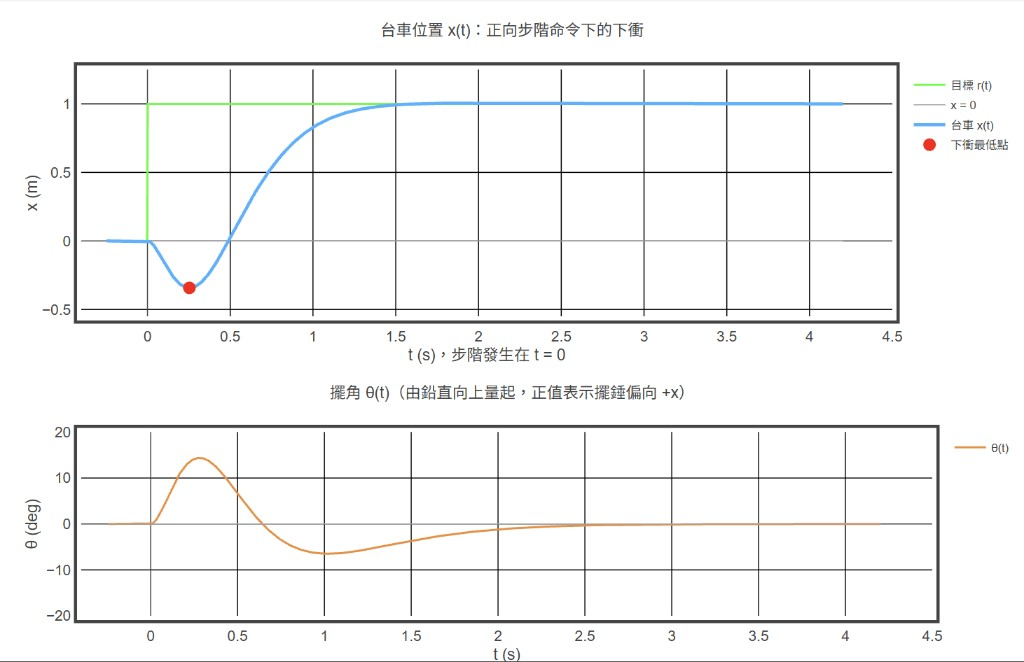
\includegraphics[width=0.92\textwidth]{sim_xt_theta.png}
  \caption{VPython 同步畫出的台車位置與擺角。\(t=0\) 命令跳到 \(+1\,\mathrm{m}\) 後，\(x\) 先降到約 \(-0.34\,\mathrm{m}\)（紅點），\(\theta\) 同時升到約 \(+14^\circ\)，之後才回到目標。}
  \label{fig:sim}
\end{figure}

\begin{figure}[ht]
  \centering
  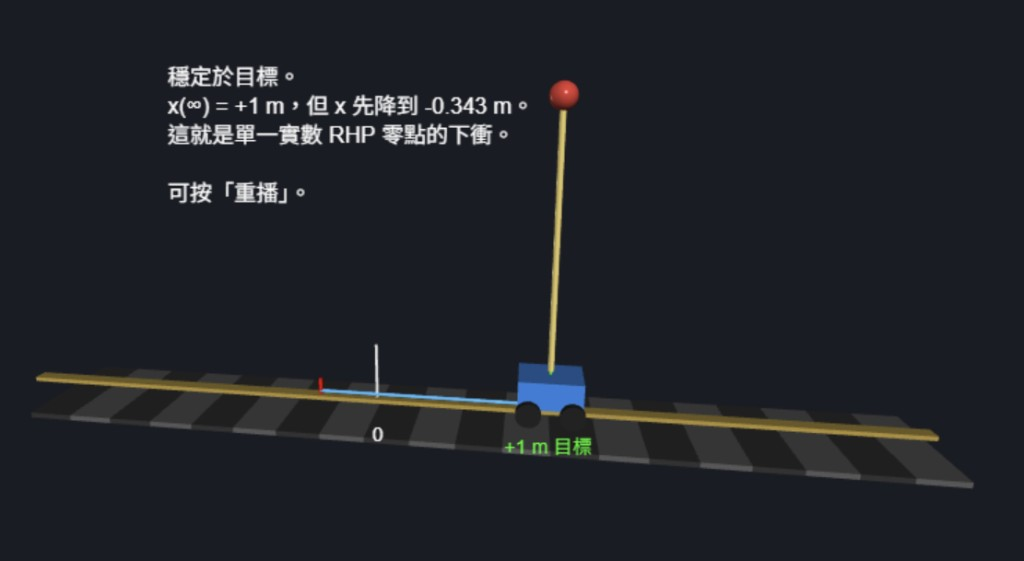
\includegraphics[width=0.88\textwidth]{sim_cart.png}
  \caption{步階結束後的三維畫面。台車停在 \(+1\,\mathrm{m}\)、擺回到直立。青色是台車軌跡，左方紅點是下衝最低點 \(x=-0.343\,\mathrm{m}\)。}
  \label{fig:cart}
\end{figure}

圖~\ref{fig:sim}、圖~\ref{fig:cart} 和上表是同一次非線性軌跡。\(x\) 在 \(t\approx 0.25\,\mathrm{s}\) 降到約 \(-0.34\,\mathrm{m}\)，之後才過原點、停在 \(+1\,\mathrm{m}\)。
\(\theta\) 的正峰值約 \(+14^\circ\)，出現在台車還在目標左側的時候；\(t\approx 1\,\mathrm{s}\) 擺角改為約 \(-6.5^\circ\)，代表台車已往右追、把擺往回拉。
全程 \(|\theta|\) 不超過約 \(14.4^\circ\)，所以線性設計和畫面上的非線性運動沒有拆開。
\(x(t)\) 先往下穿出 0，就是第 46 題 (c) 定義的下衝；它和畫面上台車先往左是同一件事。

%==============================================================================
\section{延伸三　為什麼必須先往反方向}

延伸三用延伸二的軌跡做力學說明。這裡不再證明第 46 題 (c) 的若且唯若，只用那個定理已經保證的初始方向，解釋台車為什麼非先往 \(-x\) 不可。

\subsection{步階那一瞬間畫面上有什麼}

\(t=0\) 之前系統是停的，擺是直的。命令一切成 \(+1\,\mathrm{m}\)，力立刻是 \(-57.5\,\mathrm{N}\)，箭頭指向左。
台車往 \(-x\) 滑，青色的地面軌跡也往左長。
同一段時間裡圖~\ref{fig:sim} 的 \(x(t)\) 從 0 降到負值，最低約 \(-0.34\,\mathrm{m}\)。
這條曲線先往下，就是台車本體在往遠離目標的那一側走。

擺桿同時往目標傾。\(\theta\) 的定義是擺錘相對支點偏向 \(+x\) 為正。
\(t=0.2\,\mathrm{s}\) 時台車已經在 \(-0.32\,\mathrm{m}\)，\(\theta\) 卻是 \(+13^\circ\)：支點在左，擺錘在支點右邊，也就是倒向 \(+1\,\mathrm{m}\) 那一側。
等這個傾角建立起來，力改成向右，台車折返去追擺錘，\(x(t)\) 才從谷底爬起來，最後和 \(\theta\) 一起收到 \((x,\theta)=(1,0)\)。

\subsection{慣性與力矩}

擺錘沒有被外力直接推。水平方向的外力只加在台車上，擺錘只能靠桿子受力。

剛下命令時 \(\theta=\dot\theta=0\)。把 \eqref{eq:lin-th} 寫成
\begin{equation}
  \ddot\theta=\frac{g}{L}\theta-\frac{1}{L}\ddot x,
  \label{eq:thdd}
\end{equation}
在 \(t=0^+\) 有 \(\theta=0\)，所以 \(\ddot\theta(0^+)=-\ddot x(0^+)/L\)。
要讓 \(\theta\) 變成正的（擺先倒向目標），必須 \(\ddot\theta(0^+)>0\)，也就是 \(\ddot x(0^+)<0\)。
支點得先往左加速。擺錘的水平速度不能跳變，支點往左跑，擺錘就落在支點右側。這就是畫面上 \(\theta\) 先變正、\(x\) 先變負。

\(\theta>0\) 之後，重力項 \((g/L)\theta\) 和 \(\theta\) 同號。正立是位能最高的地方，重力不會把擺扶正，只會讓它更往右側倒。
這時再把台車往 \(+x\) 加速：支點追過擺錘，\(\ddot x>0\) 在 \eqref{eq:thdd} 裡提供負的角加速度，把 \(\theta\) 收回 0，同時整個系統的淨位移往目標走。
表裡 \(t=0.2\,\mathrm{s}\) 力已經轉正，但 \(x\) 還在負的，就是「傾角已經夠了，開始追」的那一段。

重心也一起先往左。水平外力決定的是系統質心的加速度，\(F(0^+)<0\) 代表質心一開始往 \(-x\) 加速。
質心比台車更靠擺錘那邊：
\[
  x_{\mathrm{cm}}=x+\frac{mL}{M+m}\sin\theta.
\]
這段 \(\theta>0\)，擺錘在台車右側，所以台車比質心更左，\(x\) 的下衝比質心更深。
最後 \(\theta=0\)、\(x=+1\) 時質心也在 \(+1\,\mathrm{m}\)。質心最後要往右，是靠後來那段正的力把一開始往左的動量補回來；第一步的力仍然必須是負的，否則傾角的符號是錯的。

\subsection{如果沒有這一下反向}

若步階一到就讓 \(\ddot x(0^+)\ge 0\)，則 \(\ddot\theta(0^+)\le 0\)，\(\theta\) 立刻變負。
擺錘落在支點左側，倒離目標。
接著 \((g/L)\theta<0\)，重力把 \(|\theta|\) 越拉越大，擺往錯誤的一側倒下。

這個平衡點要的是 \(x=+1\) 而且 \(\theta=0\)、角速度為 0。
台車若在 \(\theta\) 仍是負的時候停住，\eqref{eq:thdd} 裡重力項還在把擺往下拉，停不在直立。
要把已經變負的 \(\theta\) 拉回來，仍然需要一段 \(\ddot x<0\)，也就是台車還是得往反方向加速，只是換到更後面、而且傾角已經變大。
線性模型能用的範圍只有十幾度；等擺明顯倒向錯誤側，這個平衡就離開了。

所以反向不是這組增益碰巧造成的。
\(T(0)>0\) 而 \(\ddot x(0^+)=N<0\) 被零點 \(\sqrt{g/L}\) 固定住：只要極點留在左半平面、直流增益為正，步階的第一下都是往 \(-x\)。
不做這一下，擺的傾角符號與目標相反，重力會把它帶離直立，到不了「台車在 \(+1\,\mathrm{m}\)、擺是直的」那個狀態。

\end{document}
